\documentclass[11pt]{report}

\usepackage{hyperref}
\usepackage{graphicx} %Package f�r Grafiken
\usepackage{subfig} % Package f�r mehrere Grafiken nebeneinander
\usepackage{amsmath}
\DeclareMathOperator{\atantwo}{atan2}

%Zeilenabstand
\linespread{1.5}

%graphics
\usepackage{graphicx}
\usepackage[margin=01in,includefoot]{geometry}
\usepackage{fancyhdr}
\usepackage{float}

% citation
\usepackage{apacite} % APA Citation
\usepackage{natbib} % Additional bibtex commands

\begin{document}
\chapter{Date Cleaning and Preparation}

\section{New York Inspection Data}

The main dataset for our project is retrieved from the \href{https://data.ny.gov/Economic-Development/Retail-Food-Store-Inspections-Current-Ratings/d6dy-3h7r}{official site of the State of New York}. It contains a total of 28'300 A to C ratings from of food store inspections. When we downloaded the data on the XXX it has been the version of June 26, 2019 with observations from March 2018 to March 2019. \\
\\
The data published by the state of New York includes not only a list of all the food ratings of different shops but also part of the history of the inspection grade development. This means the same shops could appear several times with different issues. To avoid the problem of having the identical shop more than one time we ordered the dataset ascending to the inspection date. Considering only the newest entry of every shop would have led to a bias regarding the hygiene grade because the bad graded shops improved themselves. Thus we decided to only take in account the oldest entry of every shop.\\
\\
Our analysis predicts the food store inspection ratings from this dataset for the City of New York. This includes the counties New York, Kings, Bronx, Richmond and Queens. We decided to focus on city level only because covariate data is vastly available there. In addition the distribution of classes is highly imbalanced on state level which can be slightly diminished by focusing on city data only.

\section{Chain Information}

The data set reveals not only the shops trade name but also its owner. This enabled us to identify if the shop is part of a chain. We added this parameter beside to the number of shops which belong to the specific chain. It seems possible to have an impact on the hygiene grade if the shop is part of a bigger chain. 

\section{Spatial Data}

Some of the predictors rely on geolocation data. The cleaned inspection dataset contains spatial information in form of latitude and longitude data for most of the observations. The latitude and longitude information, however, is embedded in a larger address string. We create a function to extract the location data in two new columns. A check for \texttt{NA} values reveals that 748 values missing location information. The exact address is available for all shops though. Therefore, we combine, street, city and ZIP code to a single string that can be used with the Google Maps API\footnote{In essence, the Google Maps API is a free service offered by Google. It requires only a one-time registration with a valid email address. Afterwards, it generates an API Key that must be included in the R-script  with the command \texttt{register\_google(key = "API KEY")}.} to obtain the missing latitude and longitude details. A Map of the completed data is illustrated in Figure~\ref{map1} on state and city level.\\
\begin{figure}
\captionof{figure}{Geographic Distribution of the inspected Shops \label{map1}} 
\subfloat[New York State]{%
       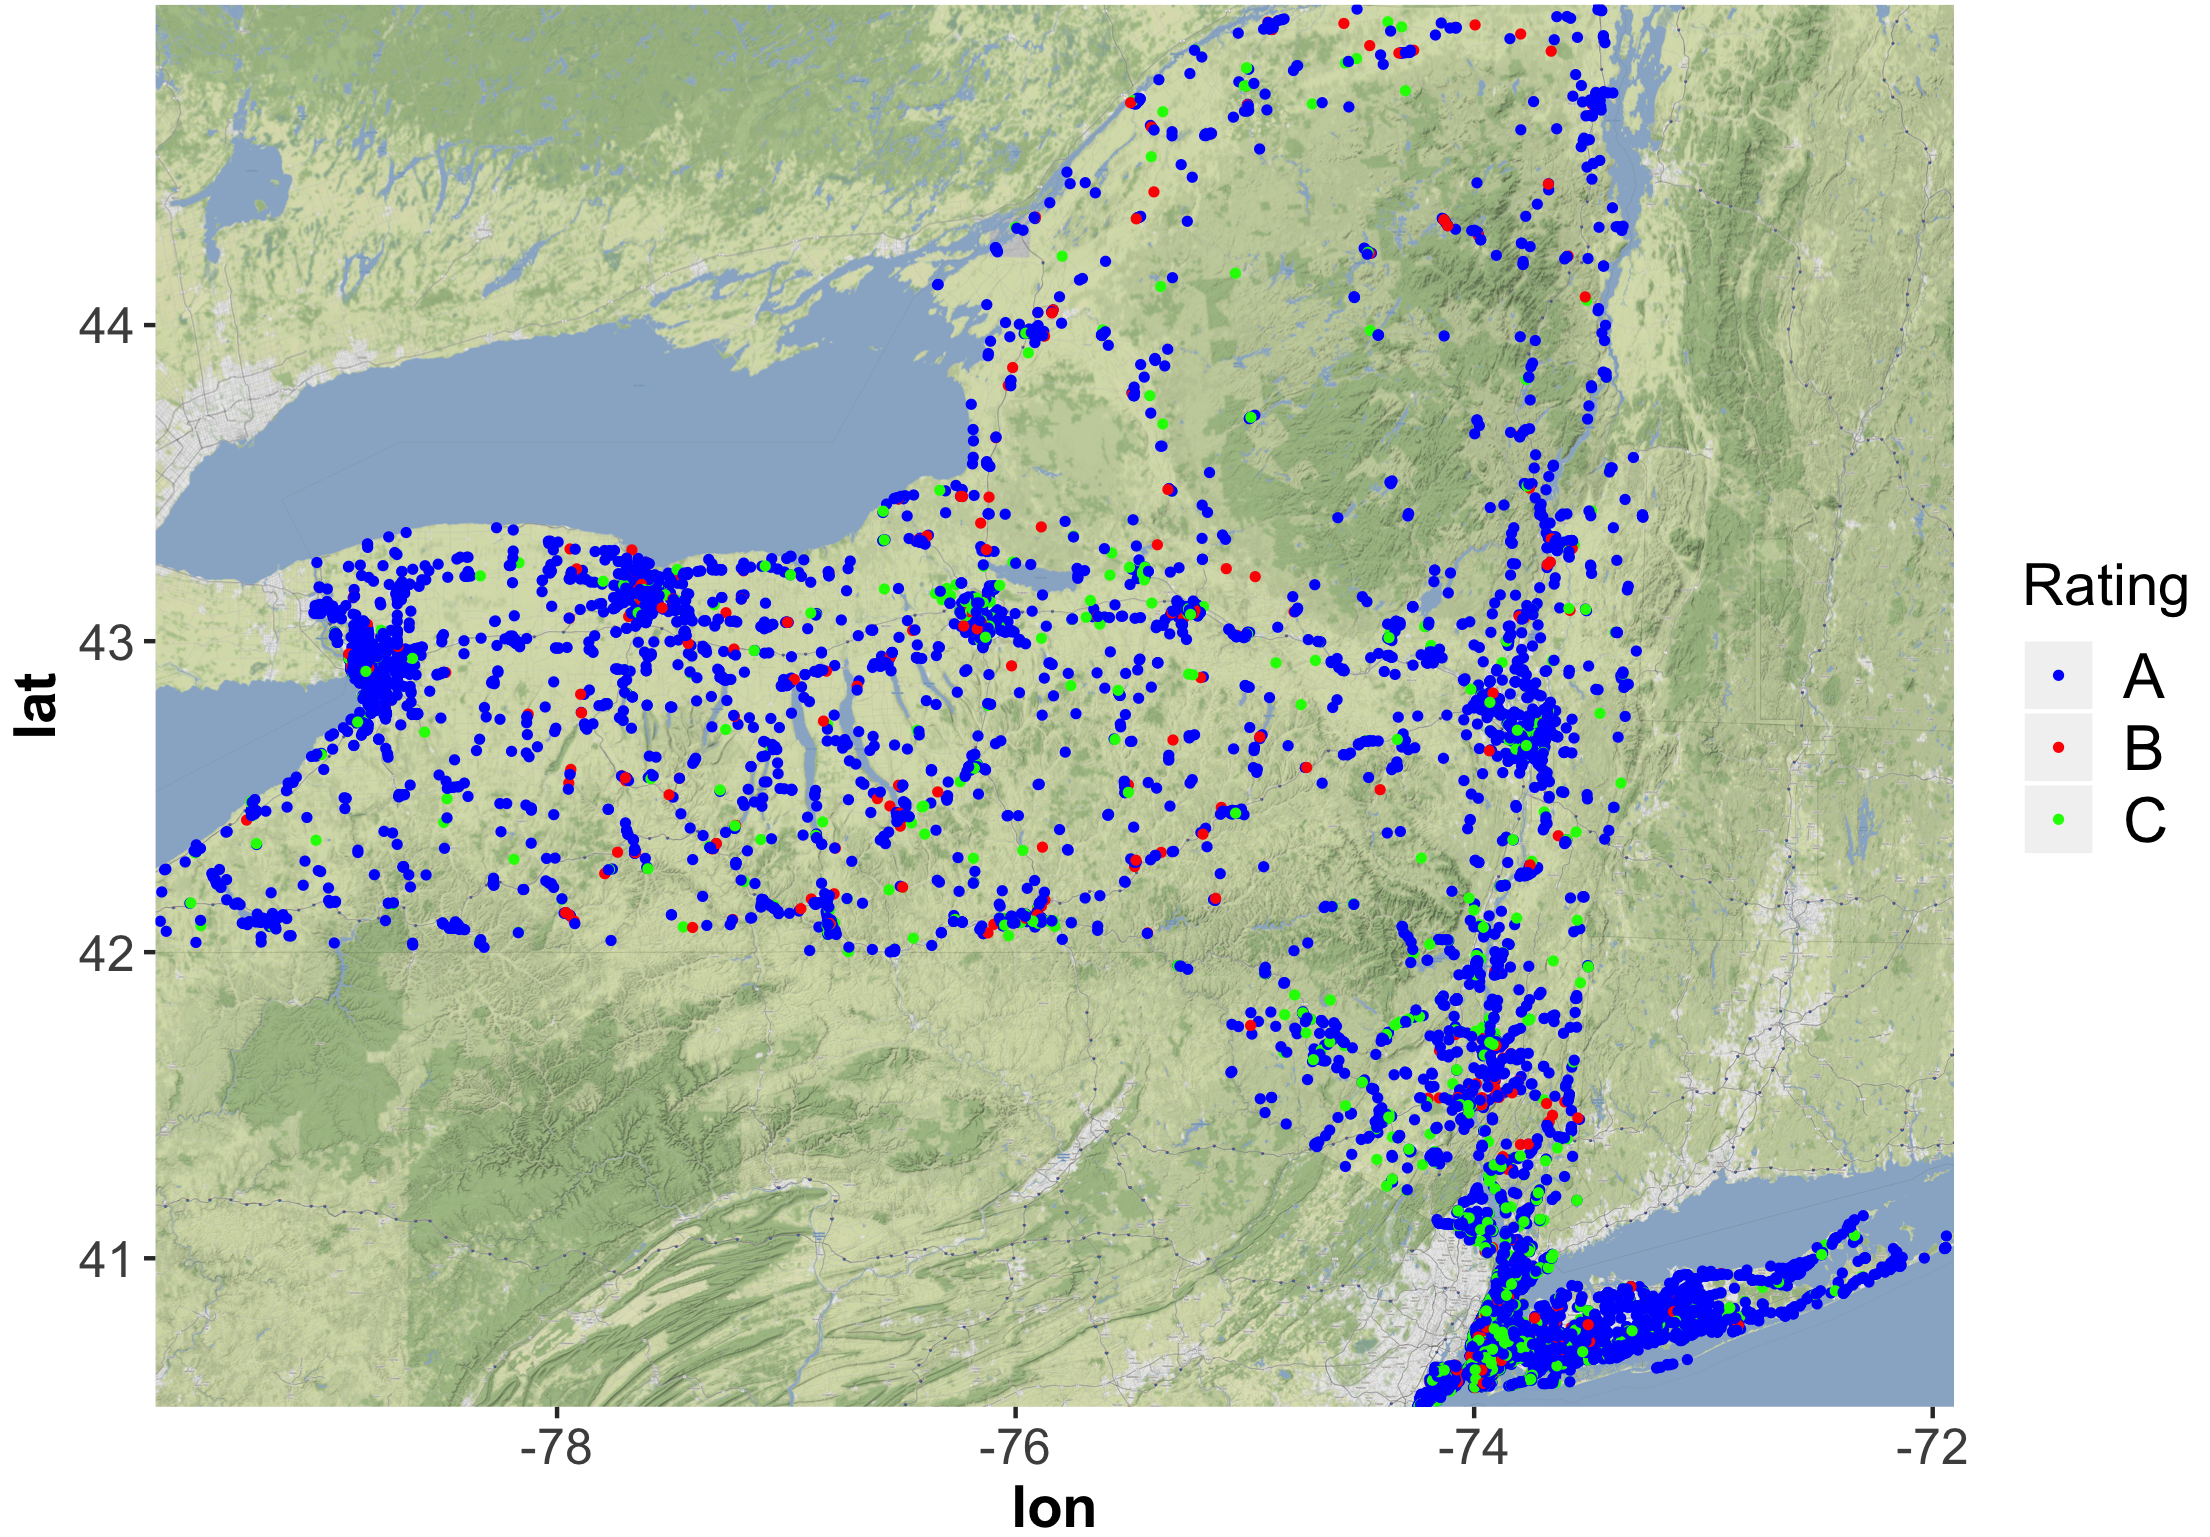
\includegraphics[width=0.5\textwidth]{Plots/Plot1_Map.png}
     }
     \hfill
     \subfloat[New York City]{%
       \includegraphics[width=0.5\textwidth]{Plots/Plot2_Map.png}
     }
\end{figure}
With complete spatial information, we now compute the two variables "shops density in 1km radius" as well as "rating of the closest neighbor". To get the distances of coordinates in meters, we apply the Haversine Formula\footnote{The Haversine Formula has its roots in spherical trigonometry and calculates the geodesic distance -- the shortest path between two points on a curved surface of a sphere, like the Earth. It needs to be mentioned that Haversine Formula does not take into account changes in altitude \citep[pp. 157 - 160]{haversine}. However, it provides sufficient accuracy for the scope of this project.}
\begin{equation} a = \sin^{2}(\frac{\Delta\alpha}{2}) + \cos(\alpha_{1})\cos(\alpha_{2})\sin^{2}(\frac{\Delta\lambda}{2})  \end{equation}
\begin{equation} d = R \left( 2 \atantwo (\sqrt{a}, \sqrt{1-a} )  \right) \end{equation}
where $\alpha_{i}$ are latitudes, $\lambda_{i}$ are longitudes, $R$ is the earth's radius ($6371\times10^{3}m$).

\section{Subway Data}

In a next step, we amend our New York City inspection data with location information of subway stations. We use again \href{https://data.ny.gov/Transportation/NYC-Transit-Subway-Entrance-And-Exit-Data/i9wp-a4ja}{an official dataset provided by the State of New York}. The dataset contains the location of every subway entrance and its corresponding station. We are only interested in the station. Therefore, we remove all duplicates of stations with multiple entrances and then use again the Haversine Formula to find the distance of the closest station to every shop.

\section{Google Web Scraper}

While doing research to find datasets with regards to food inspections we decided to gather more information from webpages. The reviews from customers, written on google places, could give us information about how individual persons have experienced their visit to the specific food shop. In order to gather this information from the internet we set up a web scraper. We used the package \textit{RSelenium} to execute an automated google search for all the food shops. This included a lot of trial and error due to unforeseen changes of the xPaths and other errors. A very fast but costly alternative would have been to use the Google Places API which provides access to all information stored by Google Places. Although it takes much more time we decided to go ahead with scraping the data ourselves. In terms of time a lot of patience was needed. Most of the errors only showed up in the middle of the scraping process, which had a duration of about 24 hours for all the food shops. Unfortunately most of the errors occurred towards the end of the scraping. Therefore, it was only possible to adjust the function after the script run during the night. This resulted in a lot of waiting and adjusting but finally the data was scraped successfully. Nonetheless the scraped data was not in a useable format yet. After tidying and joining the data to the original dataset it was ready to be used. \\

A brief analysis of the dataset revealed the incompleteness of the ratings. Approximately 40\% of the shops don't have an entry in google places and thus neither rating. After a lot of discussion on how to handle the problem we agreed on using the number of reviews as a parameter of the internet popularity. 

\section{Airbnb Data}

In order to acquire additional data and parameters on the location of the shops, we integrated data from Airbnb (average price and number of rooms). To join the original and the airbnb data frames a matching key is needed. Regarding the dataset only longitude and latitude were available. Therefore we used the above mentioned spatial data to assign the respective parameter to the ZIP codes in New York. Thereafter we grouped the data by ZIP code, calculated the respective means and counts and added it to the new tibble.

\chapter{Data Analysis}

\section{The Class Imbalance Problem}
Closer scrutiny of Figure~\ref{map1} sheds light on the extremely imbalanced distribution of the original data. In fact, the rating A contributes to XX\% on state level while B and C are only represented to XX\% and XX\% respectively. This differences in the occurrence has a large impact on the prediction capabilities of a model. The univariate linear discriminant analysis can perfectly illustrate the issue. The decision rule
\begin{equation*}\delta_{k}(x) = x \frac{\mu_{k}}{\sigma^{2}} - \frac{\mu_{k}^{2}}{2\sigma^{2}} + log(\pi_{k})\end{equation*}
with the decision boundary for two classes equal to
\begin{equation*}\delta_{1}(x) = \delta_{2}(x) \Leftrightarrow x = \frac{\mu_{1} + \mu_{2}}{2} + log\left(\frac{\pi_2}{\pi_{1}}\right)\frac{\sigma^{2}}{\mu_{1} - \mu_{2}}.\end{equation*}
If the two classes are perfectly equally represented, the prior probabilities are $\pi_{1} = \pi_{2}$ and the $\log$ term gets zero. In the presence of highly skewed classes, in turn, $\pi_{1}$ and $\pi_{2}$ are different from each other. If class 1 occurs more often it holds that $\lim_{x \to 0^{+}}log(x) = -\infty \Leftrightarrow \lim_{\pi_{1} \to 1 (\pi_{2} \to 0^{+})}log(\frac{\pi_{2}}{\pi_{1}}) = -\infty$. So, the following three extreme cases for decision boundaries can be distinguished:
\begin{align*} x = \lim_{\pi_{1} \to 1} \frac{\mu_{1} + \mu_{2}}{2} -\infty \qquad  x = \frac{\mu_{1} + \mu_{2}}{2} \text{ with } \pi_1 = \pi_2 \qquad x = \lim_{\pi_{1} \to 0^{+}} \frac{\mu_{1} + \mu_{2}}{2} -\infty \end{align*}
Hence, the decision boundary is equal to the average mean of the covariate among the two classes for perfectly symmetrically distributed classes. If the two classes are imbalanced, in turn, the decision boundary moves infinitely to the right or to the left. As a consequence, the model will simply always predict the class that is heavily overrepresented and ignore the others. The methodology presented in the next chapter will exactly address this issue and, hence, improve the prediction accuracy of inspection grades B and C.

\section{Analysis Methodology}

Our approach to overcome the Class Imbalance Problem is related to bagging. \citet[p. ]{James} use bagging to reduce the variance in tree models. However, instead of taking a random subset of the entire data like in bagging, we use repeated subsets that show an equal distribution of the three classes. Therefore, we either take more observations from the B or C class known as oversampling or we apply undersampling and take only a part of the observations from the A class. \citet[p. 83]{imbalance} outlines that both approaches have drawbacks. While oversampling increases the likelihood for overfitting since we create exact copies of a minority class, undersampling ignores potentially useful data points. To address these weaknesses, we combine over- and undersampling with bagging which results in over- and under-bagging. According to \citet[pp. 174 - 176]{imbalance}, over- and under-bagging represent strong methods to overcome an imbalance issue that are relatively simple to implement. We combine this approach with a forward-stepwise-selection that is suggested by \citet[p. ]{James}. In detail, we created our own model selection algorithm that processes the following steps:
\begin{enumerate}
\item Take a subset of the data where the three classes are balanced either with over- or undersampling
\item Divide the subset in K equally sized folds for K-Fold Cross-Validation (CV)
\item Use nine folds as training data to estimate the model with one variable for each p variables
\item Use the remaining fold as testing data to make predictions
\item Calculate the rate of wrong predictions
\item Repeat step X to Y until all folds are used as testing data (K times)
\item Calculate the average of all error rates and take the model with the lowest CV error
\item Add one additional variable and apply step X to Y again
\item Repeat the entire process B times and then take the average rate of the CV error to get the bagged-CV-errors
\end{enumerate}
After we found the model with the lowest bagged-CV-error, we estimate the model B times and then we take majority vote of all the B models to classify the observation to one of the three categories.

\section{Pre-Analysis Variable Elimination}
The obvious drawback of the described methodology is that it is computationally intensive. Using all XX variables would be accordingly difficult given the extent of this project. A boosting model with 100 variables, for instance, would run for XX hours. Furthermore, some of the demographic variables are anyways linear combinations of each other and must be excluded from our analysis. For the remaining ones, we calculate the correlation to the Inspection Grade we want to predict and take the 20 covariates with the highest correlation.



\chapter{Conclusion}
--> Wrong predictors


\newpage

\bibliographystyle{apacite}
\bibliography{bibliography}

\end{document}